\documentclass[11pt,letterpaper]{article}
\usepackage[margin=2.5cm]{geometry}
\usepackage[utf8]{inputenc}
\usepackage[T1]{fontenc}
\usepackage{lmodern}
\usepackage{amsmath,amssymb,amsthm,mathtools,bm}
\usepackage{enumitem}
\usepackage{booktabs}
\usepackage{tikz}
\usetikzlibrary{arrows.meta,patterns,positioning,calc}
\usepackage{pgfplots}
\pgfplotsset{compat=1.16}
\usepackage{titlesec}
\usepackage[hidelinks]{hyperref}

\setlength{\parindent}{0pt}
\setlength{\parskip}{0.5em}
\titleformat{\section}{\large\bfseries}{\thesection.}{0.6em}{}
\titleformat{\subsection}{\normalsize\bfseries}{\thesubsection.}{0.6em}{}

\theoremstyle{definition}
\newtheorem{definition}{Definition}[section]
\newtheorem{example}{Example}[section]
\newtheorem{exercise}{Exercise}[section]
\newtheorem{theorem}{Theorem}[section]
\newtheorem{remark}{Remark}[section]

\newcommand{\R}{\mathbb{R}}
\newcommand{\N}{\mathbb{N}}
\newcommand{\Z}{\mathbb{Z}}
\newcommand{\U}{\mathcal{U}}
\newcommand{\E}{\mathbb{E}}
\newcommand{\Var}{\operatorname{Var}}
\newcommand{\Cov}{\operatorname{Cov}}
\newcommand{\Normal}{\mathcal{N}}
\newcommand{\dd}{\,\mathrm{d}}
\newcommand{\T}{^{\top}}
\renewcommand{\P}{P}
\newcommand{\set}[1]{\left\{#1\right\}}
\newcommand{\given}{\mid}
\newcommand{\note}[1]{\textit{#1}}

\title{Lecture 3: Random Variables}
\author{}\date{}

\begin{document}
\maketitle

\section{Random variables}
For a sample space $\Omega = \set{\omega_1, \dots, \omega_n}$, a \emph{random variable} is a mapping or rule
\[
X : \Omega \to \R
\]
that assigns a real number $X(\omega_i)$ to each outcome $\omega_i \in \Omega$.

The \emph{range} of $X$, denoted $R_X$ or $\operatorname{Range}(X)$, is the set of all possible values that $X$ can take.

\begin{example}
For a random experiment, a coin is flipped five times. The sample space for this experiment is
\[
\Omega = \set{CCCCC, CCCCS, CCCSS, \dots, SSSSS},
\]
with $C$ for ``cara'' (heads) and $S$ for ``sello'' (tails), and $|\Omega| = 2^5 = 32$.
If we are interested in the number of $C$s, then we can define a random variable $X$ such that
\[
X(CCCCC) = 5, \qquad X(CCCCS) = 4, \qquad \dots
\]
and so on. What is the range of $X$? \ $R_X = \set{0,1,2,3,4,5}$.

What is the probability of $X = 2$? Since $P(A) = |A|/|\Omega|$, we need $|A|$ for the event $A$ of having two $C$s. Placing the three $S$s, the two $C$s can go into the $4$ gaps around them either in different gaps, $\binom{4}{2} = \frac{4!}{2!\,2!} = 6$ ways, or both in the same gap ($CC$), $4$ ways. Thus $|A| = 10$ and therefore
\[
P(X = 2) = \frac{10}{32}.
\]
Basically, one needs a table:
\begin{center}
\begin{tabular}{c|cccccc}
$x$ & 0 & 1 & 2 & 3 & 4 & 5\\ \hline
$P(X=x)$ & $\frac{1}{32}$ & $\frac{5}{32}$ & $\frac{10}{32}$ & $\frac{10}{32}$ & $\frac{5}{32}$ & $\frac{1}{32}$
\end{tabular}
\end{center}
with
\[
\sum_{x=0}^{5} P(X = x) = \sum_{x=0}^{5} P_X(x) = 1.
\]
\end{example}

\begin{example}
Let us suppose that someone buys two electronic components. Each electronic component can be either acceptable ($a$) or defective ($d$). We have that
\[
\Omega = \set{(d,d), (d,a), (a,d), (a,a)},
\]
with probabilities
\[
P((d,d)) = 0.09, \quad P((d,a)) = 0.21, \quad P((a,d)) = 0.21, \quad P((a,a)) = 0.49.
\]
Let $X$ be the random variable representing the number of acceptable components. Determine $R_X$:
\begin{center}
\begin{tabular}{c|ccc}
$x$ & 0 & 1 & 2\\ \hline
$P(X=x)$ & $0.09$ & $0.42$ & $0.49$
\end{tabular}
\end{center}
where $P(X=1) = P(A)$ with $A = \set{(d,a), (a,d)}$.
\end{example}

\subsection{Types of random variables}
There are two types of random variables:
\begin{itemize}
\item \textbf{Discrete:} $R_X$ is countable, meaning there is a one-to-one correspondence between $R_X$ and (a subset of) the set of natural numbers.
\item \textbf{Continuous:} $R_X$ is uncountable.
\end{itemize}

\begin{example}
Flip a coin twice and let $X$ be the number of ``caras''. Then
\[
\Omega = \set{SS, CS, SC, CC}, \qquad R_X = \set{0,1,2},
\]
\begin{center}
\begin{tabular}{c|ccc}
$x$ & 0 & 1 & 2\\ \hline
$P(X=x)$ & $\frac14$ & $\frac12$ & $\frac14$
\end{tabular}
\qquad\qquad
\begin{tikzpicture}[baseline=(current bounding box.center),x=1cm,y=2.4cm]
\draw[->] (-0.3,0) -- (2.8,0) node[right] {$x$};
\draw[->] (0,0) -- (0,1.15) node[above] {$P(X=x)$};
\foreach \x/\p in {0.5/0.25, 1.3/0.5, 2.1/0.25} {\draw[thick] (\x,0) -- (\x,\p); \fill (\x,\p) circle (1.5pt);}
\node[below] at (0.5,0) {0}; \node[below] at (1.3,0) {1}; \node[below] at (2.1,0) {2};
\foreach \y in {0.25,0.5,1} {\draw (-0.05,\y) -- (0.05,\y) node[left=3pt] {\small $\y$};}
\end{tikzpicture}
\end{center}
\end{example}

%=====================================================
\section{Probability mass function (PMF)}
For a discrete random variable $X$, $P(X = x)$ is called a \emph{probability (mass) function}.

\textbf{Properties:}
\begin{enumerate}[label=(\roman*)]
\item $P(X = x) \ge 0$,
\item $\sum_{x \in R_X} P(X = x) = 1$,
\item for $A \subseteq R_X$, $P(X \in A) = \sum_{x \in A} P(X = x)$.
\end{enumerate}

\begin{homework}{2}
Two six-sided dice are rolled. Let $X$ be the sum of the two results. Find
\begin{enumerate}[label=(\roman*)]
\item the range $R_X$ of $X$;
\item the probability mass function $P(X = x)$ for each $x \in R_X$.
\end{enumerate}

\soln
\begin{enumerate}[label=(\roman*)]
\item The smallest sum is $1 + 1 = 2$ and the largest is $6 + 6 = 12$, and every value in between can occur: $R_X = \set{2, 3, \dots, 12}$.
\item The sample space $\Omega = \set{(d_1, d_2) : d_1, d_2 \in \set{1, \dots, 6}}$ has $36$ equally likely outcomes, so $P(X = x) = |\set{X = x}|/36$. Counting the pairs with $d_1 + d_2 = x$:
\begin{center}
\begin{tabular}{c|ccccccccccc}
$x$ & 2 & 3 & 4 & 5 & 6 & 7 & 8 & 9 & 10 & 11 & 12\\ \hline
$36\,P(X = x)$ & 1 & 2 & 3 & 4 & 5 & 6 & 5 & 4 & 3 & 2 & 1
\end{tabular}
\end{center}
For example, $\set{X = 5} = \set{(1,4), (2,3), (3,2), (4,1)}$, so $P(X = 5) = 4/36$, as in Lecture 2. In one formula,
\[
P(X = x) = \frac{6 - |x - 7|}{36}, \qquad x = 2, \dots, 12,
\]
and indeed $\sum_{x} P(X = x) = \frac{1 + 2 + 3 + 4 + 5 + 6 + 5 + 4 + 3 + 2 + 1}{36} = \new{\frac{36}{36}} = 1$.
\end{enumerate}
\end{homework}

%=====================================================
\section{Cumulative distribution function (CDF)}
\[
F_X : \R \to [0,1], \qquad F_X(x) = P(X \le x).
\]
For the cumulative, we break down $R_X$ in parts. First, notice that with $A = \set{x' \mid x' \le x}$,
\[
F_X(x) = P(X \le x) = P(X \in A) = \sum_{x' \in A} P(X = x') = \sum_{x_k \le x} P(X = x_k).
\]
For the previous example (two coin flips):
\[
F_X(0) = P(X \le 0) = 0.25, \qquad F_X(1) = \sum_{x=0}^{1} P(X=x) = 0.75, \qquad F_X(2) = \sum_{x=0}^{2} P(X=x) = 1,
\]
\[
F_X(x) =
\begin{cases}
0 & x < 0,\\
1/4 & 0 \le x < 1,\\
3/4 & 1 \le x < 2,\\
1 & 2 \le x.
\end{cases}
\qquad
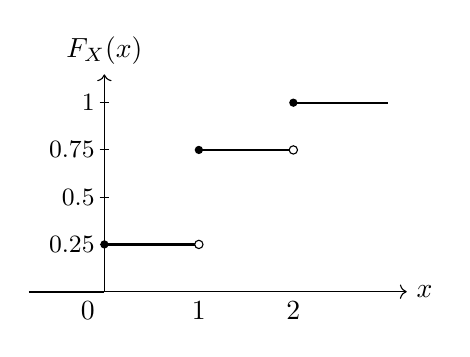
\begin{tikzpicture}[baseline=(current bounding box.center),x=1.2cm,y=2.4cm]
\draw[->] (-0.8,0) -- (3.2,0) node[right] {$x$};
\draw[->] (0,0) -- (0,1.15) node[above] {$F_X(x)$};
\draw[thick] (-0.8,0) -- (0,0);
\draw[thick] (0,0.25) -- (1,0.25); \fill (0,0.25) circle (1.5pt); \draw[fill=white] (1,0.25) circle (1.5pt);
\draw[thick] (1,0.75) -- (2,0.75); \fill (1,0.75) circle (1.5pt); \draw[fill=white] (2,0.75) circle (1.5pt);
\draw[thick] (2,1) -- (3,1); \fill (2,1) circle (1.5pt);
\foreach \y in {0.25,0.5,0.75,1} {\draw (-0.05,\y) -- (0.05,\y); \node[left] at (0,\y) {\small $\y$};}
\node[below] at (1,0) {1}; \node[below] at (2,0) {2}; \node[below left] at (0,0) {0};
\end{tikzpicture}
\]

For consecutive values $x_k < x_{k+1}$ in $R_X$,
\[
F_X(x_{k+1}) - F_X(x_k) = \sum_{x = x_0}^{x_{k+1}} P(X = x) - \sum_{x = x_0}^{x_k} P(X = x) = P(X = x_{k+1}) \ge 0,
\]
so $F_X(x_{k+1}) \ge F_X(x_k)$ (non-decreasing).

A CDF completely defines the PMF. Moreover,
\[
x \to -\infty: \ F_X(x) \to 0, \qquad x \to +\infty: \ F_X(x) \to 1.
\]

\paragraph{Probability in an interval.}
\begin{align*}
P(X \le b) &= P(X \le a) + P(a < X \le b),\\
P(a < X \le b) &= P(X \le b) - P(X \le a) = F_X(b) - F_X(a).
\end{align*}

\begin{exercise}[Exercise 2.14.2]
Plot the CDF for $P(X = 2) = P(X = 3) = 1/10$ and $P(X = 5) = 8/10$.
\[
F_X(x) =
\begin{cases}
0 & x < 2,\\
0.1 & 2 \le x < 3,\\
0.2 & 3 \le x < 5,\\
1 & 5 \le x.
\end{cases}
\qquad
\begin{tikzpicture}[baseline=(current bounding box.center),x=0.7cm,y=2.4cm]
\draw[->] (-0.5,0) -- (7,0) node[right] {$x$};
\draw[->] (0,0) -- (0,1.15) node[above] {$F_X(x)$};
\draw[thick] (2,0.1) -- (3,0.1); \fill (2,0.1) circle (1.5pt); \draw[fill=white] (3,0.1) circle (1.5pt);
\draw[thick] (3,0.2) -- (5,0.2); \fill (3,0.2) circle (1.5pt); \draw[fill=white] (5,0.2) circle (1.5pt);
\draw[thick] (5,1) -- (6.8,1); \fill (5,1) circle (1.5pt);
\foreach \x in {2,3,5} \node[below] at (\x,0) {\x};
\foreach \y in {0.5,1} {\draw (-0.05,\y) -- (0.05,\y); \node[left] at (0,\y) {\small $\y$};}
\end{tikzpicture}
\]
Then
\begin{align*}
P(2 < X \le 4.8) &= F_X(4.8) - F_X(2) = 0.2 - 0.1 = 0.1,\\
P(2 \le X \le 4.8) &= 0.1 + P(X = 2) = 0.2.
\end{align*}
\end{exercise}

%=====================================================
\section{Continuous random variables}
\subsection{Probability density function}
For continuous random variables, the CDF is defined as
\[
F_X(x) = \int_{-\infty}^{x} f_X(u)\dd u,
\]
where $F_X(x)$ satisfies the properties mentioned above. The function
\[
f_X(x) = \frac{\mathrm{d}F_X(x)}{\mathrm{d}x}
\]
is called the \emph{probability density function} (PDF).

Note that $F_X(x)$ has probability units, whereas $\mathrm{d}F_X(x)/\mathrm{d}x$ has units of probability over $\mathrm{d}x$. That's why $f_X(x)$ is a density. $F_X(x)$ needs to be continuous everywhere, and $F'_X(x) = f_X(x)$ must hold almost everywhere (wherever the derivative exists).

Notice that, as $F_X(x)$ is a non-decreasing function, then
\[
F'_X(x) = f_X(x) \ge 0, \qquad \lim_{x \to \infty} F_X(x) = 1 = \int_{-\infty}^{\infty} f_X(u)\dd u.
\]
With
\[
F_X(x) = P(X \le x) = \int_{-\infty}^{x} f_X(u)\dd u, \qquad
F_X(a) = \int_{-\infty}^{a} f_X(u)\dd u, \qquad
F_X(b) = \int_{-\infty}^{b} f_X(u)\dd u,
\]
where $b > a$, we get
\[
F_X(b) - F_X(a) = \int_{-\infty}^{b} f_X(u)\dd u - \int_{-\infty}^{a} f_X(u)\dd u
= \int_{-\infty}^{b} f_X(u)\dd u + \int_{a}^{-\infty} f_X(u)\dd u,
\]
\[
P(a < X \le b) = \int_{a}^{b} f_X(u)\dd u = F_X(b) - F_X(a).
\]

%=====================================================
\section{Discrete distributions}

\subsection{Bernoulli distribution}
$X \sim \operatorname{Bernoulli}(x;\theta)$ if
\[
P(X = x) = \theta^{x}(1-\theta)^{1-x}, \qquad x \in \set{0,1}.
\]
This is the case $n = 1$ of the binomial distribution below.

\subsection{Binomial distribution}
Let us consider a mini-experiment which can result in a failure ($F$) or a success ($S$). Then, do $n$ trials of that mini-experiment. One can wonder: what is the probability that $x$ of those $n$ experiments end up being successes?

Let us consider $n = 4$. The sample space is
\[
\Omega = \set{FFFF, SFFF, FSFF, FFSF, FFFS, SSFF, \dots}.
\]
For one success,
\[
P(X = 1) = P(A), \qquad A = \set{SFFF, FSFF, FFSF, FFFS}.
\]
If all outcomes were equally likely, $P(X=1) = |A|/|\Omega| = \binom{4}{1}|\Omega|^{-1}$ and $P(SFFF) = |\Omega|^{-1}$. But notice that $SFFF = S \cap F \cap F \cap F$; therefore
\[
P(SFFF) = P(S)\,P(F)\,P(F)\,P(F).
\]
If $P(S) = \theta$, then $P(F) = 1 - \theta$. Thus
\[
P(X = 1) = \binom{4}{1}\theta^{1}(1-\theta)^{4-1}.
\]

Experiments following $\operatorname{Bin}(\cdot)$ are called \emph{binomial experiments}. This type of experiments conform either exactly or approximately to the following requirements:
\begin{enumerate}
\item The experiment consists of a sequence of $n$ trials.
\item Each trial can result in one of two possible outcomes: success ($S$) or failure ($F$).
\item Trials are independent: the outcome of a particular trial doesn't influence the outcome of any other trial.
\item The probability of success $P(S) = \theta$ is constant from trial to trial.
\end{enumerate}
The binomial distribution is
\[
P(X = x) = \operatorname{Bin}(x; n, \theta) = \binom{n}{x}\theta^{x}(1-\theta)^{n-x},
\]
with $x$ the number of successes.

\begin{remark}
The expression above allows us to make one significant difference between Bayesian statistics and classical statistics. For Bayesian statistics we are going to write $p(y \mid \theta)$, and a distribution $p(\theta)$ is assigned to $\theta$. For frequentist statistics, $\theta$ is unknown but it is not treated as a random variable.
\end{remark}

\begin{example}
It is known that discs produced in a factory are defective with probability $0.01$, independently between them. The discs are sold in packages containing $10$ discs, and a guarantee offers a refund whenever more than one, out of ten, are defective.

(i) What is the probability of using the guarantee? We need $P(X > 1)$, with $X \sim \operatorname{Bin}(x; n, \theta)$, $n = 10$, $\theta = 0.01$:
\[
P(X > 1) = P(X \ge 2) = \sum_{x=2}^{10} \operatorname{Bin}(x; n, \theta).
\]
Easier: $P(X \le 1) + P(X > 1) = 1$, so $P(X > 1) = 1 - P(X \le 1)$, with
\[
P(X \le 1) = \sum_{x=0}^{1} \binom{10}{x} 0.01^{x}(1-0.01)^{10-x},
\]
\[
\binom{10}{0}(1-0.01)^{10} = 0.99^{10}, \qquad \binom{10}{1} 0.01^{1}(1-0.01)^{9} = 0.1\,(0.99)^{9},
\]
\[
P(X \le 1) = 0.99 \times 0.99^{9} + 0.1 \times 0.99^{9} = 0.99573,
\qquad
P(X > 1) = 0.00427 \equiv \mu.
\]

(ii) If someone buys $3$ packages, what is the probability of having exactly one package returned? With $Y \sim \operatorname{Bin}(y; 3, \mu)$,
\[
P(Y = 1) = \binom{3}{1}\mu^{1}(1-\mu)^{2} = \frac{3!}{1!\,2!}\mu(1-\mu)^2 = 3\mu(1-\mu)^2 = 0.0127.
\]
\end{example}


\begin{homework}{2}
Suppose $20\%$ of the copies of a textbook fail a binding-strength test. We pick $15$ copies at random and let $X$ be the number of copies, among the $15$, that fail the test. Find the probability that
\begin{enumerate}[label=(\roman*)]
\item exactly $8$ copies fail;
\item at most $8$ copies fail;
\item at least $8$ copies fail.
\end{enumerate}

\soln
Each copy fails independently with the same probability, so $X \sim \operatorname{Bin}(x; n = 15, \theta = 0.2)$.
\begin{enumerate}[label=(\roman*)]
\item
\[
P(X = 8) = \binom{15}{8}(0.2)^{8}(0.8)^{7} = \new{6435}\times(0.2)^{8}(0.8)^{7} \approx \new{0.0035}.
\]
\item ``At most $8$'' means $X \le 8$:
\[
P(X \le 8) = \sum_{x=0}^{8}\binom{15}{x}(0.2)^{x}(0.8)^{15-x} \approx \new{0.9992}.
\]
\item ``At least $8$'' means $X \ge 8$. As in the disc example, the complement is quicker:
\[
P(X \ge 8) = 1 - P(X \le \new{7}) = 1 - \big[P(X \le 8) - P(X = 8)\big] \approx 1 - \new{0.9958} = \new{0.0042}.
\]
\end{enumerate}
Note that (ii) and (iii) both include $X = 8$, so $P(X \le 8) + P(X \ge 8) = 1 + P(X = 8)$.
\end{homework}

\subsection{Categorical distribution}
If now we have $K$ classes, $x \in \set{1, 2, \dots, K}$, then
\[
P(X = x) = \operatorname{Cat}(x) = \theta_k \quad \text{if } x = k.
\]
More compactly,
\[
\operatorname{Cat}(x; \theta) = \prod_{j=1}^{K} \theta_j^{\delta_{xj}},
\qquad
\delta_{xj} =
\begin{cases}
0 & x \neq j,\\
1 & x = j,
\end{cases}
\qquad\text{and}\qquad \sum_{k} \theta_k = 1.
\]

\subsection{Multinomial distribution}
Let us suppose that you run an experiment consisting of $n$ trials:
\begin{itemize}
\item The outcome of each trial can be any one of $K$ classes (indexed by $\alpha = 1, \dots, K$).
\item $x_\alpha$ represents the number of trials (out of $n$) whose outcome landed in the class $\alpha$.
\end{itemize}
Then, the probability of having $x_1, x_2, \dots, x_K$ is
\[
M(x_1, \dots, x_K; \theta_1, \dots, \theta_K) = \binom{n}{x_1 \cdots x_K}\prod_{\alpha=1}^{K}\theta_\alpha^{x_\alpha},
\qquad
\sum_{\alpha=1}^{K} x_\alpha = n.
\]

\subsection{Poisson distribution}
$X \sim \operatorname{Poisson}(\lambda)$ if
\[
P(X = x) = \frac{e^{-\lambda}\lambda^{x}}{x!}, \qquad x = 0, 1, 2, \dots
\]
This distribution tells the probability of a given number of occurrences of an event within a fixed interval of time (or space, area, etc.).

\paragraph{Derivation.}
Let us consider $N(t)$: the number of times the event has happened by time $t$. So, we want to find $P_k(t) \equiv P(N(t) = k)$.

But, how do events occur over time? What happens in the interval $[t, t+h]$ when $h$ is tiny? Three possibilities:
\begin{enumerate}[label=\roman*.]
\item Nothing happens.
\item Exactly one event happens.
\item Two or more events happen.
\end{enumerate}
Writing $\alpha > 0$ for the rate of occurrence and $o(h)$ for terms that vanish faster than $h$, for $h \to 0$:
\begin{align*}
P\big(N([t,t+h]) = 1\big) &\approx \alpha h,\\
P\big(N([t,t+h]) \ge 2\big) &= o(h),\\
P\big(N([t,t+h]) = 0\big) &= 1 - \alpha h - o(h).
\end{align*}
There are two ways for $k$ events to occur by time $t+h$:
\begin{enumerate}[label=(\roman*)]
\item By time $t$, $k$ events happened, and nothing happened during $[t, t+h]$. Then
\[
P_k^{(i)}(t+h) = P_k(t)\times(1 - \alpha h - o(h)).
\]
\item By time $t$, $k-1$ events happened, and one happened during $[t,t+h]$:
\[
P_k^{(ii)}(t+h) = P_{k-1}(t)\times \alpha h.
\]
\end{enumerate}
Then
\begin{align*}
P_k(t+h) &= P_k(t)\times(1 - \alpha h) + P_{k-1}(t)\times \alpha h + o(h),\\
P_k(t+h) \new{{}- P_k(t)} &= -\alpha h\,P_k(t) + \alpha h\,P_{k-1}(t) + o(h),\\
\frac{P_k(t+h) - P_k(t)}{\new{h}} &= -\alpha P_k(t) + \alpha P_{k-1}(t) + \new{\frac{o(h)}{h}}.
\end{align*}
If $h \to 0$,
\[
\new{\frac{\mathrm{d}P_k(t)}{\mathrm{d}t}} = -\alpha P_k(t) + \alpha P_{k-1}(t).
\]

\begin{itemize}
\item For $k = 0$:
\[
\frac{\mathrm{d}P_0(t)}{\mathrm{d}t} = -\alpha P_0(t) \ \Rightarrow\ P_0(t) = \new{C e^{-\alpha t}}.
\]
At $t = 0$ the probability of observing $k = 0$ is $1$: $P_0(t=0) = 1 = C$. As we wait longer, the probability of $k = 0$ (``observing nothing'') vanishes. Thus, for $t \to \infty$, $P_0(t) \to 0$.

\item For $k = 1$:
\[
\frac{\mathrm{d}P_1(t)}{\mathrm{d}t} = -\alpha P_1(t) + \alpha P_0(t) = -\alpha P_1(t) + \alpha \new{e^{-\alpha t}},
\qquad
\frac{\mathrm{d}P_1(t)}{\mathrm{d}t} \new{{}+ \alpha P_1(t)} = \alpha e^{-\alpha t}.
\]
Using $\frac{\mathrm{d}}{\mathrm{d}t}[u(t)v(t)] = \dot u(t)v(t) + u(t)\dot v(t)$, multiply by $u(t)$:
\[
\new{u(t)}\frac{\mathrm{d}P_1(t)}{\mathrm{d}t} + \alpha \new{u(t)}P_1(t) = \alpha \new{u(t)}e^{-\alpha t},
\]
and choose $\dot u(t) = \alpha u(t)$, i.e.\ $u(t) = e^{\alpha t}$:
\[
\new{e^{\alpha t}}\frac{\mathrm{d}P_1(t)}{\mathrm{d}t} + \alpha \new{e^{\alpha t}}P_1(t) = \alpha \new{e^{\alpha t}}e^{-\alpha t} = \new{\alpha}
\ \Rightarrow\
\new{\frac{\mathrm{d}}{\mathrm{d}t}\big[e^{\alpha t}P_1(t)\big]} = \alpha.
\]
Integrating,
\[
\int \mathrm{d}t\,\frac{\mathrm{d}}{\mathrm{d}t}\big[e^{\alpha t}P_1(t)\big] = \alpha\int \mathrm{d}t
\ \Rightarrow\
e^{\alpha t}P_1(t) = \new{\alpha t + C}
\ \Rightarrow\
P_1(t) = (\alpha t + C)\new{e^{-\alpha t}}.
\]
At $t = 0$: $P_1(0) = \alpha\times 0 + C = 0$, so $C = 0$. Thus
\[
P_1(t) = \alpha t\, e^{-\alpha t}.
\]
\end{itemize}
Continuing in this way, with $\lambda = \alpha t$ and $X = N(t)$,
\[
P(X = k) = \frac{e^{-\alpha t}(\alpha t)^{k}}{k!}.
\]
Here, $t$ represents the length of a time window over which we are counting how many events occur.

\paragraph{Assumptions of the Poisson distribution.}
Assume that an interval is divided into a very large number of equal subintervals so that the probability of the occurrence of an event in any subinterval is very small. With that, we need the following assumptions:
\begin{enumerate}
\item The probability of the occurrence of an event is constant for all subintervals.
\item There can be no more than one occurrence in each subinterval.
\item Occurrences are independent; an occurrence in one interval doesn't influence the probability of occurrence in another interval.
\end{enumerate}

\begin{example}
The distribution of the amount of emails that someone receives in a work day can be modeled with a Poisson distribution. On average, someone receives $\alpha = 0.2$ emails per minute.

What is the probability of receiving no emails in a $5$-minute interval?
\[
P(X = 0) = e^{-\alpha t}, \qquad \text{at } t = 5: \quad P(X=0) = e^{-0.2\times 5} = e^{-1}.
\]
What is the probability of receiving more than $3$ emails in a $10$-minute interval?
\[
P(X > 3) + P(X \le 3) = 1 \ \Rightarrow\ P(X > 3) = 1 - P(X \le 3),
\qquad
P(X \le 3) = \sum_{k=0}^{3}\frac{e^{-\alpha t}(\alpha t)^k}{k!}.
\]
With $\alpha t = 2$:
\[
P(X \le 3) = e^{-2} + \frac{e^{-2}\times 2}{1!} + \frac{e^{-2}\times 2^2}{2!} + \frac{e^{-2}\times 2^3}{3!}
= e^{-2}\left(1 + 2 + 2 + \frac43\right) = e^{-2}\times\frac{19}{3} = 0.857,
\]
\[
P(X > 3) = 1 - 0.857 = 0.143.
\]
\end{example}

%=====================================================
\section{Continuous distributions}

\subsection{Uniform distribution}
$X \sim \operatorname{Uniform}(a,b)$ if
\[
f_X(x) =
\begin{cases}
\dfrac{1}{b-a} & \text{for } x \in [a,b],\\[4pt]
0 & \text{otherwise}.
\end{cases}
\]
The CDF for $f_X(x)$ is
\[
F_X(x) = \int_{-\infty}^{x} f_X(u)\dd u = \int_{a}^{x} f_X(u)\dd u
=
\begin{cases}
0 & \text{if } x < a,\\[2pt]
\dfrac{x-a}{b-a} & \text{if } x \in [a,b),\\[4pt]
1 & \text{if } x \ge b.
\end{cases}
\]
\begin{center}
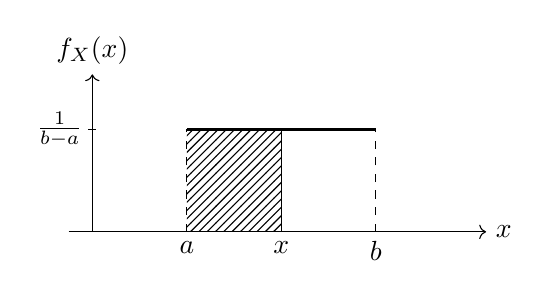
\begin{tikzpicture}[x=1cm,y=1cm]
\draw[->] (-0.3,0) -- (5,0) node[right] {$x$};
\draw[->] (0,0) -- (0,2) node[above] {$f_X(x)$};
\fill[pattern=north east lines] (1.2,0) rectangle (2.4,1.3);
\draw[thick] (1.2,1.3) -- (3.6,1.3);
\draw[dashed] (1.2,0) -- (1.2,1.3); \draw[dashed] (3.6,0) -- (3.6,1.3); \draw (2.4,0) -- (2.4,1.3);
\node[below] at (1.2,0) {$a$}; \node[below] at (2.4,0) {$x$}; \node[below] at (3.6,0) {$b$};
\node[left] at (0,1.3) {$\frac{1}{b-a}$}; \draw (-0.05,1.3) -- (0.05,1.3);
\end{tikzpicture}
\end{center}

\subsection{Exponential distribution}
$X \sim \operatorname{Exp}(\lambda)$ if
\[
f_X(x) =
\begin{cases}
\lambda e^{-\lambda x} & \text{if } x > 0,\\
0 & \text{if } x \le 0.
\end{cases}
\]
Equivalently, with $\lambda = 1/\beta$, \ $f_X(x) = \frac{1}{\beta}e^{-x/\beta}$.

\textbf{CDF:}
\[
F_X(x) = \int_{-\infty}^{x}\lambda e^{-\lambda u}\dd u = \int_{0}^{x}\lambda e^{-\lambda u}\dd u.
\]
Since $\frac{\mathrm{d}e^{-\lambda u}}{\mathrm{d}u} = -\lambda e^{-\lambda u}$,
\[
\int_0^x \lambda e^{-\lambda u}\dd u = -e^{-\lambda u}\Big|_0^x = -(e^{-\lambda x} - 1) = 1 - e^{-\lambda x}.
\]

The Poisson distribution gives the probability of an event occurring a number of times during a time window (a period of certain length). On the other hand, waiting times between events follow an exponential distribution.

\paragraph{Memorylessness.}
\[
P(T > t + s \mid T > s) = P(T > t).
\]

\begin{example}[Continuation of the previous example]
(i) Find the probability of a waiting time of more than $10$ minutes for the next email to come in. With $\alpha = 0.2$ and $F(t) = 1 - e^{-\alpha t}$,
\[
P(T \le 10) + P(T > 10) = 1,
\qquad
P(T > 10) = 1 - (1 - e^{-\alpha t}) = e^{-\alpha t} = e^{-0.2\times 10} = e^{-2}.
\]
Also, $F(2) = 1 - e^{-0.4}$.
\end{example}

\subsection{Normal distribution}
$X \sim \Normal(\mu, \sigma^2)$, with $\mu$ the (population) average and $\sigma^2$ the variance:
\[
f_X(x) = \frac{1}{\sigma\sqrt{2\pi}}\exp\left\{-\frac{(x-\mu)^2}{2\sigma^2}\right\},
\qquad
F_X(x) = \int_{-\infty}^{x}\frac{1}{\sigma\sqrt{2\pi}}\exp\left\{-\frac{(s-\mu)^2}{2\sigma^2}\right\}\dd s.
\]
\begin{center}
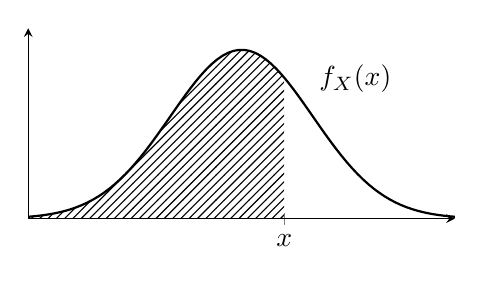
\begin{tikzpicture}
\begin{axis}[width=7cm,height=4cm,axis lines=left,xtick={0.6},xticklabels={$x$},ytick=\empty,domain=-3:3,samples=80,ymin=0,ymax=0.45,xlabel={},ylabel={}]
\addplot[pattern=north east lines,draw=none,domain=-3:0.6] {exp(-x^2/2)/sqrt(2*pi)} \closedcycle;
\addplot[thick] {exp(-x^2/2)/sqrt(2*pi)};
\node at (axis cs:1.6,0.33) {$f_X(x)$};
\end{axis}
\end{tikzpicture}
\end{center}

\paragraph{Standardization.}
If $X \sim \Normal(\mu,\sigma^2)$, then
\[
Z = \frac{X - \mu}{\sigma} \sim \Normal(0,1).
\]
Thus,
\[
P(a < X < b) = P\left(\frac{a-\mu}{\sigma} < Z < \frac{b-\mu}{\sigma}\right).
\]
The CDF of $Z$ is denoted $\Phi$, so $F_X(x) = \Phi\big(\frac{x-\mu}{\sigma}\big)$.

%=====================================================
\section{Bivariate distributions}

\subsection{Discrete variables: joint PMF}
\textbf{Notation:} joint probability
\[
P(X = x, Y = y) = P(x,y).
\]
\textbf{Range:}
\[
R_{XY} \subseteq R_X \times R_Y = \set{(x,y) \mid x \in R_X \wedge y \in R_Y}.
\]
\textbf{Properties:}
\[
\sum_{(x,y) \in R_{XY}} P(X = x, Y = y) = 1.
\]
For $A \subseteq \R^2$,
\[
P\big((X,Y) \in A\big) = \sum_{(x,y)} P(X = x, Y = y),
\]
where $(x,y) \in (A \cap R_{XY})$.

Since $X = x$ is $\set{(x_i, y_j) \mid x_i = x \wedge y_j \in R_Y}$ and $Y = y$ is $\set{(x_i, y_j) \mid x_i \in R_X \wedge y_j = y}$, then
\[
P(X = x, Y = y) = P\big((X = x) \cap (Y = y)\big).
\]

\paragraph{Law of total probability.}
Since $A = A \cap \Omega$, for any partition $\Omega = \bigcup_{i=1}^{n} B_i$ we have
\[
A = A \cap \bigcup_{i=1}^{n} B_i = \bigcup_{i=1}^{n}(A \cap B_i).
\]
For instance, $A \cap (B_1 \cup B_2) = (A \cap B_1) \cup (A \cap B_2)$, and with $B_1 \cap B_2 = \emptyset$,
\[
(A \cap B_1) \cap (A \cap B_2) = A \cap \underbrace{(B_1 \cap B_2)}_{\emptyset} = \emptyset.
\]
Thus $P(A) = \sum_{i=1}^{n} P(A \cap B_i)$. This leads to the \emph{marginal PMFs}:
\[
P(X = x) = \sum_{j} P(X = x, Y = y_j), \qquad P(Y = y) = \sum_{i} P(X = x_i, Y = y).
\]

Bivariate joint PMFs can be described using tables:
\begin{center}
\begin{tabular}{c|ccc|c}
 & $Y=0$ & $Y=1$ & $Y=2$ & \\ \hline
$X=0$ & $\frac16$ & $\frac14$ & $\frac18$ & $\frac{13}{24}$\\[2pt]
$X=1$ & $\frac18$ & $\frac16$ & $\frac16$ & $\frac{11}{24}$\\ \hline
 & $\frac{7}{24}$ & $\frac{5}{12}$ & $\frac{7}{24}$ &
\end{tabular}
\end{center}
For example, $P(X=0, Y=0) = 1/6$, $P(X=1, Y=2) = 1/6$, \dots

\textbf{Marginals:}
\begin{align*}
P(X = 0) &= \sum_{j=1}^{3} P(X = 0, Y = y_j) = P(X=0, Y=y_1) + P(X=0, Y=y_2) + P(X=0, Y=y_3)\\
&= P(X=0, Y=0) + P(X=0, Y=1) + P(X=0, Y=2) = \frac16 + \frac14 + \frac18 = \frac16 + \frac38 = \frac{26}{48}.
\end{align*}
Same for $P(X = 1)$. For $P(Y = 0)$ one has
\[
P(Y = 0) = \sum_{i=1}^{2} P(X = x_i, Y = 0) = P(X=0, Y=0) + P(X=1, Y=0) = \frac16 + \frac18 = \frac{14}{48} = \frac{7}{24}.
\]

\begin{itemize}
\item Find $P(X = 0, Y \le 1)$:
\begin{align*}
P(X = 0, Y \le 1) &= \sum_{x_i \in \set{0}}\ \sum_{y_j \in \set{0,1}} P(X = x_i, Y = y_j)\\
&= \sum_{x_i \in \set{0}}\big(P(X = x_i, Y = 0) + P(X = x_i, Y = 1)\big)\\
&= P(X=0, Y=0) + P(X=0, Y=1) = \frac16 + \frac14 = \frac{10}{24} = \frac{5}{12}.
\end{align*}
\item Find $P(Y = 1 \mid X = 0)$:
\[
P(Y = 1 \mid X = 0) = \frac{P(Y = 1, X = 0)}{P(X = 0)} = \frac{1/4}{13/24} = \frac{24}{52} = \frac{12}{26} = \frac{6}{13}.
\]
\end{itemize}

\subsection{Bivariate CDF}
\[
F(x,y) = P(X \le x, Y \le y) = P\big((X \le x) \cap (Y \le y)\big).
\]
\textbf{Properties:}
\begin{align*}
F(x) &= \lim_{y \to \infty} F(x,y) = P(X \le x), & F(y) &= \lim_{x \to \infty} F(x,y) = P(Y \le y),\\
F(\infty,\infty) &= 1, & F(-\infty, y) &= 0 \ \text{for any } y, \qquad F(x, -\infty) = 0 \ \text{for any } x.
\end{align*}

\begin{center}
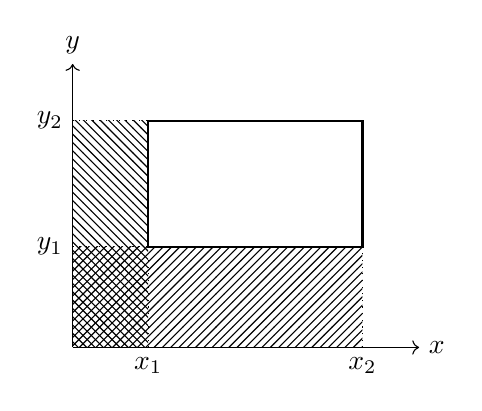
\begin{tikzpicture}[scale=0.8]
\draw[->] (0,0) -- (5.5,0) node[right] {$x$};
\draw[->] (0,0) -- (0,4.5) node[above] {$y$};
\fill[pattern=north west lines] (0,0) rectangle (1.2,3.6);
\fill[pattern=north east lines] (0,0) rectangle (4.6,1.6);
\draw[thick] (1.2,1.6) rectangle (4.6,3.6);
\draw[dotted] (0,3.6) -- (1.2,3.6); \draw[dotted] (0,1.6) -- (1.2,1.6);
\draw[dotted] (1.2,0) -- (1.2,1.6); \draw[dotted] (4.6,0) -- (4.6,1.6);
\node[below] at (1.2,0) {$x_1$}; \node[below] at (4.6,0) {$x_2$};
\node[left] at (0,1.6) {$y_1$}; \node[left] at (0,3.6) {$y_2$};
\end{tikzpicture}
\end{center}
\begin{align*}
P(x_1 < X \le x_2,\ y_1 < Y \le y_2) &= P(X \le x_2, Y \le y_2) - P(X \le x_2, Y \le y_1)\\
&\quad - P(X \le x_1, Y \le y_2) + P(X \le x_1, Y \le y_1)\\
&= F(x_2, y_2) - F(x_2, y_1) - F(x_1, y_2) + F(x_1, y_1).
\end{align*}
For $x_1 \to -\infty$ and $y_1 \to -\infty$: \ $P(X \le x_2, Y \le y_2) = F(x_2, y_2)$.

\subsection{Continuous random variables}
A function $f_{XY}(x,y)$ is called the \emph{joint PDF} of $X$ and $Y$ if
\begin{enumerate}[label=(\roman*)]
\item $f_{XY}(x,y) \ge 0$,
\item $\displaystyle\int_{-\infty}^{\infty}\int_{-\infty}^{\infty} f_{XY}(x,y)\dd x\dd y = 1$,
\item $\displaystyle P(x_1 \le X \le x_2,\ y_1 \le Y \le y_2) = \int_{x_1}^{x_2}\int_{y_1}^{y_2} f_{XY}(x,y)\dd y\dd x$.
\end{enumerate}
\textbf{Marginals:}
\[
f_X(x) = \int_{-\infty}^{\infty} f_{XY}(x,y)\dd y, \qquad f_Y(y) = \int_{-\infty}^{\infty} f_{XY}(x,y)\dd x.
\]
\textbf{Independence:} $X$ and $Y$ are independent if
\[
f_{XY}(x,y) = f_X(x)\,f_Y(y).
\]
\textbf{Conditional distributions:}
\[
f_{X|Y}(x \mid y) = \frac{f_{XY}(x,y)}{f_Y(y)}.
\]

\begin{example}
\[
f(x,y) =
\begin{cases}
1 & \text{if } 0 \le x \le 1,\ 0 \le y \le 1,\\
0 & \text{otherwise}.
\end{cases}
\]
Find $P(X \le 1/2, Y \le 1/2)$:
\[
P(X \le 1/2, Y \le 1/2) = \int_0^{1/2}\int_0^{1/2}\dd x\dd y = \int_0^{1/2}\dd x\int_0^{1/2}\dd y = \frac12\times\frac12 = \frac14.
\]
\end{example}

\begin{example}
\[
f(x,y) =
\begin{cases}
x + y & 0 \le x \le 1,\ 0 \le y \le 1,\\
0 & \text{otherwise}.
\end{cases}
\]
Check:
\begin{align*}
\int_0^1\int_0^1 (x+y)\dd x\dd y &= \int_0^1\dd y\int_0^1\dd x\,(x+y)
= \int_0^1\dd y\new{\left(\frac12 x^2 + yx\right)\Big|_0^1}
= \int_0^1\dd y\left(\new{\left(\frac12 + y\right) - 0}\right)\\
&= \new{\left(\frac12 y + \frac12 y^2\right)\Big|_0^1} = \new{\frac12 + \frac12} = 1.
\end{align*}
Find $P(X < 1/4 \mid Y = 1/3)$. We need $f_{X|Y}(x \mid y) = f_{XY}(x,y)/f_Y(y)$, with
\[
f_Y(y) = \int_0^1 (x+y)\dd x = \int_0^1 x\dd x + \int_0^1 y\dd x = \frac12 x^2\Big|_0^1 + yx\Big|_0^1 = \frac12 + y,
\qquad
f_{X|Y}(x \mid y) = \frac{x+y}{y + \frac12}.
\]
Then
\begin{align*}
P(X < 1/4 \mid Y = 1/3) &= \int_0^{1/4}\frac{x + 1/3}{\frac13 + \frac12}\dd x
= \int_0^{1/4}\frac{x + 1/3}{\new{5/6}}\dd x
= \int_0^{1/4}\frac{\new{(3x+1)/3}}{5/6}\dd x
= \int_0^{1/4}\new{\frac{2(3x+1)}{5}}\dd x\\
&= \new{0.4}\left(\new{\int_0^{1/4}3x\dd x + \int_0^{1/4}\dd x}\right)
= 0.4\left(\new{\frac32 x^2\Big|_0^{1/4}} + \new{x\Big|_0^{1/4}}\right)\\
&= 0.4\left(\new{\frac32\cdot\frac{1}{2^4}} + \new{\frac14}\right)
= \frac{0.4}{4}\left(\frac{3}{2^3} + 1\right) = 0.1\left(\frac38 + 1\right) = \frac{0.1\times 11}{8} = \frac{1.1}{8}.
\end{align*}
\end{example}

%=====================================================
\section{Functions of random variables}
Suppose a random variable $X$. Let $Y = g(X)$ be a transformation of $X$. How to find $P(Y = y)$?

For discrete variables we do
\[
P(Y = y) = P(g(X) = y) = P(X = g^{-1}(y)).
\]
This is, we want the table of $Y$ from the table of $X$. For example, taking $Y = X^2$ with
\begin{center}
\begin{tabular}{c|ccc}
$x$ & $-1$ & $0$ & $1$\\ \hline
$P(X=x)$ & $\frac14$ & $\frac12$ & $\frac14$
\end{tabular}
\quad$\Rightarrow$\quad
\begin{tabular}{c|ccc}
$y = x^2$ & $1$ & $0$ & $1$\\ \hline
$P(X = g^{-1}(y))$ & $\frac14$ & $\frac12$ & $\frac14$
\end{tabular}
\end{center}
so $P(Y = 0) = \frac12$ and $P(Y = 1) = \frac14 + \frac14 = \frac12$.

For continuous variables we work on the CDF. Given $Y = g(X)$ (with $g$ increasing),
\[
F_Y(y) = P(Y \le y) = P(g(X) \le y) = P(X \le g^{-1}(y)),
\]
for a given $R_X$. Then
\[
f_Y(y) = \frac{\mathrm{d}F_Y(y)}{\mathrm{d}y}.
\]
\begin{exercise}
$f_X(x) = e^{-x}$, \ $Y(X) = \log(X)$.
\end{exercise}

%=====================================================
\section{Expected values}

\begin{definition}[Expected value]
\textbf{Discrete variables:}
\[
\E(X) = \sum_{i=1}^{n} x_i\,P(X = x_i).
\]
\textbf{Continuous variables:}
\[
\E(X) = \int x\,f_X(x)\dd x.
\]
\end{definition}

\paragraph{Properties.}
If $X_1, X_2, \dots$ are random variables and $a_1, a_2, \dots$ constants, then
\[
\E\Big(\sum_i a_i X_i\Big) = \sum_i a_i\,\E(X_i).
\]
Indeed, writing $x^{(\ell)}$ for the values in $R_{X_i}$,
\[
\E(a_i X_i) = \sum_{\ell} a_i x^{(\ell)}\,P(X_i = x^{(\ell)}) = a_i\sum_{\ell} x^{(\ell)}\,P(X_i = x^{(\ell)}) = a_i\,\E(X_i),
\]
and, summing over the joint PMF and using the marginals,
\[
\E\Big(\sum_i a_i X_i\Big) = \sum_{x_1,\dots,x_n}\Big(\sum_i a_i x_i\Big)P(X_1 = x_1, \dots, X_n = x_n)
= \sum_i a_i\sum_{x_i} x_i\,P(X_i = x_i) = \sum_i a_i\,\E(X_i).
\]
If $X_1, \dots, X_n$ are independent, then
\[
\E\Big(\prod_{i=1}^{n} X_i\Big) = \prod_{i=1}^{n}\E(X_i).
\]

\begin{example}[Binomial]
\[
\E(X) = \sum_{x=0}^{n} x\binom{n}{x}\theta^{x}(1-\theta)^{n-x} = \sum_{x=0}^{n} x\,\frac{n!}{x!\,(n-x)!}\theta^{x}(1-\theta)^{n-x}.
\]
Using
\[
\frac{x\,n!}{x\,(x-1)!\,(n-x)!} = \frac{n\,(n-1)!}{(x-1)!\,(n-x)!},
\]
and noting that the term $x = 0$ vanishes,
\[
\E(X) = n\sum_{x=1}^{n}\binom{n-1}{x-1}\theta^{x}(1-\theta)^{n-x} = n\theta\sum_{x=1}^{n}\binom{n-1}{x-1}\theta^{x-1}(1-\theta)^{n-x}.
\]
With $N = n-1$, $y = x-1$ (so $N - y = n - x$):
\[
\E(X) = n\theta\sum_{y=0}^{N}\binom{N}{y}\theta^{y}(1-\theta)^{N-y} = n\theta.
\]
\end{example}

\paragraph{For functions.}
\[
\E(g(X)) = \sum_i g(x_i)\,P(X = x_i), \qquad \E(g(X)) = \int g(x)\,f_X(x)\dd x.
\]

%=====================================================
\section{Variance}
\[
\Var(X) = \E\big((X - \underbrace{\E(X)}_{\mu_X})^2\big).
\]
\begin{align*}
\Var(X) &= \sum_i (x_i - \mu)^2 P(X = x_i) = \sum_i \new{(x_i^2 - 2x_i\mu + \mu^2)}P(X = x_i)\\
&= \new{\sum_i} x_i^2 P(X = x_i) - 2\mu\new{\sum_i} x_i P(X = x_i) + \mu^2\new{\sum_i} P(X = x_i)\\
&= \new{\E(X^2)} - \new{2\mu^2} + \new{\mu^2} = \E(X^2) - \new{\mu^2}.
\end{align*}

\paragraph{Properties.}
\begin{enumerate}[label=(\roman*)]
\item If $a$ and $b$ are constants, then $\Var(aX + b) = a^2\Var(X)$. With $Y = aX + b$:
\begin{align*}
\Var(Y) &= \E(Y^2) - \E(Y)^2 = \E(Y^2) - \new{(a\E(X) + b)^2}\\
&= \E(\new{a^2X^2 + 2abX + b^2}) - \new{\big(a^2\E(X)^2 + 2ab\E(X) + b^2\big)}\\
&= \new{a^2\E(X^2) - a^2\E(X)^2} = \new{a^2\Var(X)}.
\end{align*}
\item If $X_1, \dots, X_n$ are independent and $a_1, \dots, a_n$ are constants, then
\[
\Var\Big(\sum_i a_i X_i\Big) = \sum_i a_i^2\Var(X_i).
\]
Indeed,
\[
\Var\Big(\sum_i a_i X_i\Big) = \E\Big(\Big(\sum_i a_i X_i - \sum_i a_i\E(X_i)\Big)^2\Big) = \E\Big[\Big(\sum_i a_i(X_i - \E(X_i))\Big)^2\Big],
\]
and, using $\big(\sum_{i=1}^{n} z_i\big)^2 = \sum_{i=1}^{n} z_i^2 + 2\sum_{i<j} z_i z_j$, the cross terms vanish for independent variables since $\E[(X_i - \E X_i)(X_j - \E X_j)] = \E(X_i - \E X_i)\,\E(X_j - \E X_j) = 0$.
\end{enumerate}


\begin{homework}{3}
Let $Y \sim \operatorname{Bin}(n, \theta)$, with PMF
\[
P(Y = y) = \binom{n}{y}\theta^{y}(1-\theta)^{n-y}, \qquad y = 0, 1, \dots, n.
\]
Show that
\begin{enumerate}[label=(\roman*)]
\item the distribution is normalized, $\sum_{y=0}^{n} P(Y = y) = 1$;
\item $\E[Y] = n\theta$;
\item $\Var(Y) = n\theta(1-\theta)$.
\end{enumerate}

\soln
\begin{enumerate}[label=(\roman*)]
\item By the binomial theorem, $(a + b)^n = \sum_{y=0}^{n}\binom{n}{y}a^{y}b^{n-y}$. With $a = \theta$ and $b = 1 - \theta$,
\[
\sum_{y=0}^{n}\binom{n}{y}\theta^{y}(1-\theta)^{n-y} = \big(\theta + (1 - \theta)\big)^{n} = \new{1}^{n} = 1.
\]
\item This is the example in the section on expected values: $\E[Y] = n\theta$.
\item It is easier to find $\E[Y(Y-1)]$ first and then use $\E[Y^2] = \E[Y(Y-1)] + \E[Y]$. The terms $y = 0$ and $y = 1$ vanish, and
\[
y(y-1)\binom{n}{y} = \frac{y(y-1)\,n!}{y!\,(n-y)!} = \new{n(n-1)}\frac{(n-2)!}{\new{(y-2)!}\,(n-y)!} = n(n-1)\binom{n-2}{y-2}.
\]
Then, with $N = n - 2$ and $k = y - 2$ (so $N - k = n - y$),
\begin{align*}
\E[Y(Y-1)] &= n(n-1)\sum_{y=2}^{n}\binom{n-2}{y-2}\theta^{y}(1-\theta)^{n-y}
= n(n-1)\new{\theta^2}\sum_{k=0}^{N}\binom{N}{k}\theta^{k}(1-\theta)^{N-k}\\
&= n(n-1)\theta^2 \cdot \new{1},
\end{align*}
where the last sum is a $\operatorname{Bin}(N, \theta)$ PMF summed over its range, which is $1$ by part (i). Therefore
\begin{align*}
\Var(Y) &= \E[Y^2] - \E[Y]^2 = \E[Y(Y-1)] + \E[Y] - \E[Y]^2\\
&= n(n-1)\theta^2 + n\theta - n^2\theta^2 = \new{n\theta - n\theta^2} = n\theta(1 - \theta).
\end{align*}
\end{enumerate}
Alternatively, $Y = \sum_{i=1}^{n} X_i$ with independent $X_i \sim \operatorname{Bernoulli}(\theta)$, $\Var(X_i) = \theta(1-\theta)$, and the property $\Var\big(\sum_i X_i\big) = \sum_i \Var(X_i)$ gives the same result in one line.
\end{homework}

%=====================================================
\section{Covariance}
\begin{align*}
\Cov(X,Y) &= \E\big((X - \mu_X)(Y - \mu_Y)\big) = \E(\new{XY - \mu_Y X - \mu_X Y + \mu_X\mu_Y})\\
&= \new{\E(XY)} - \mu_Y\underbrace{\new{\E(X)}}_{\mu_X} - \mu_X\underbrace{\new{\E(Y)}}_{\mu_Y} + \mu_X\mu_Y
= \E(XY) - \new{\E(X)\,\E(Y)},
\end{align*}
with
\[
\E(XY) = \sum_x\sum_y xy\,P(X = x, Y = y), \qquad
\E(g(X,Y)) = \sum_x\sum_y g(x,y)\,P(X = x, Y = y).
\]

%=====================================================
\section*{References}
\begin{itemize}
\item Wasserman, L. (2004). \emph{All of Statistics: A Concise Course in Statistical Inference}. Springer. Chapters 2--3: random variables, common distributions, joint and conditional distributions, expectation, variance and covariance.
\item Pishro-Nik, H. (2014). \emph{Introduction to Probability, Statistics, and Random Processes}. Kappa Research. \url{https://www.probabilitycourse.com/} Chapters 3--5: discrete and continuous random variables and joint distributions; Section 11.1: the Poisson process.
\end{itemize}

\end{document}
